\documentclass[aspectratio=169,11pt]{beamer}
\usepackage[T1]{fontenc}
\usepackage{lmodern,amsmath,amssymb,mathtools,bm,booktabs,array,graphicx,tikz}
\usetikzlibrary{arrows.meta,positioning,calc,decorations.pathreplacing,patterns}
\definecolor{ink}{HTML}{17344D}\definecolor{accent}{HTML}{087E8B}\definecolor{pale}{HTML}{EDF5F5}\definecolor{gold}{HTML}{AD6B19}
\providecommand{\dd}{\,\mathrm{d}}\providecommand{\R}{\mathbb{R}}
\providecommand{\E}{\mathbb{E}}\providecommand{\Var}{\operatorname{Var}}
\providecommand{\Cov}{\operatorname{Cov}}\providecommand{\diag}{\operatorname{diag}}
\providecommand{\norm}[1]{\left\lVert#1\right\rVert}
\providecommand{\abs}[1]{\left|#1\right|}
\usefonttheme{professionalfonts}
\setbeamercolor{normal text}{fg=black,bg=white}
\setbeamercolor{frametitle}{fg=ink,bg=white}
\setbeamercolor{title}{fg=ink}\setbeamercolor{structure}{fg=accent}
\setbeamercolor{block title}{fg=ink,bg=pale}\setbeamercolor{block body}{fg=black,bg=pale!40}
\setbeamercolor{alerted text}{fg=accent}
\setbeamerfont{frametitle}{size=\Large,series=\bfseries}
\setbeamerfont{title}{size=\LARGE,series=\bfseries}
\setbeamertemplate{navigation symbols}{}
\setbeamersize{text margin left=.7cm,text margin right=.7cm}
\setbeamertemplate{frametitle}{\vspace{.18cm}\insertframetitle\par\vspace{.1cm}{\color{accent}\hrule height .6pt}\vspace{.12cm}}
\newcommand{\notestarget}{notes.pdf}\newcommand{\noteslabel}{Notes}
\setbeamertemplate{footline}{\hspace{.7cm}\color{ink}\scriptsize Mathematical Cardiology\quad\href{\notestarget}{\noteslabel}\hfill\insertframenumber\,/\,\inserttotalframenumber\hspace{.7cm}\vspace{.18cm}}
\setbeamercovered{invisible}
\hypersetup{pdfauthor={Zan Ahmad},pdftitle={Resistance, compliance, and the reservoir equation},pdfpagemode=UseNone}
\begin{document}
\begin{frame}[plain]\vfill
{\small\color{accent} Mathematical Cardiology \quad Lecture 2}\par\medskip
{\raggedright\hyphenpenalty=10000\exhyphenpenalty=10000\LARGE\bfseries\color{ink} Resistance, compliance, and the reservoir equation}\par\bigskip
Zan Ahmad\par\smallskip
{\small Fall 2023}\par\vfill\end{frame}
\renewcommand{\notestarget}{notes.pdf\#note-two-pressure-differences-and-two-constitutive-laws}
\begin{frame}[t,fragile,label=slide-transmission-and-storage]{Transmission and storage}
\[Q=\frac{P_{\rm in}-P_{\rm out}}R,\qquad \Delta V=C\Delta P_{\rm tm}.\]\pause{} The first equation describes transport along a pathway. The second describes expansion across a wall.
\end{frame}
\renewcommand{\notestarget}{notes.pdf\#note-two-pressure-differences-and-two-constitutive-laws}
\begin{frame}[t,fragile,label=slide-transmural-pressure]{Transmural pressure}
\[P_{\rm tm}=P-P_{\rm ext}.\]\pause{} Equal endpoint pressures can give zero resistive flow and nonzero vessel distension.
\end{frame}
\renewcommand{\notestarget}{notes.pdf\#note-two-pressure-differences-and-two-constitutive-laws}
\begin{frame}[t,fragile,label=slide-compliance-and-its-units]{Compliance and its units}
\[V=V_d+C(P-P_{\rm ext}).\]\pause{}\[[C]=\mathrm{mL/mmHg}.\]\pause{} At fixed $C$ and $P_{\rm ext}$,\[V_{n+1}-V_n=C(P_{n+1}-P_n).\]
\end{frame}
\renewcommand{\notestarget}{notes.pdf\#note-combine-storage-with-a-volume-balance}
\begin{frame}[t,fragile,label=slide-a-reservoir-with-a-prescribed-supply]{A reservoir with a prescribed supply}
\[Q_{\rm in}=I,\qquad Q_{\rm out}=\frac{P-P_o}{R}.\]\pause{} The reservoir pressure changes; the outlet pressure $P_o$ is held fixed.
\end{frame}
\renewcommand{\notestarget}{notes.pdf\#note-combine-storage-with-a-volume-balance}
\begin{frame}[t,fragile,label=slide-first-write-a-volume-balance]{First write a volume balance}
\[V_{n+1}-V_n\approx h(I-Q_{{\rm out},n}).\]\pause{}\[C(P_{n+1}-P_n)\approx h\left(I-\frac{P_n-P_o}{R}\right).\]
\end{frame}
\renewcommand{\notestarget}{notes.pdf\#note-combine-storage-with-a-volume-balance}
\begin{frame}[t,fragile,label=slide-the-explicit-pressure-update]{The explicit pressure update}
\[P_{n+1}=P_n+\frac hC\left(I-\frac{P_n-P_o}{R}\right).\]\pause{} The old pressure determines the approximate outflow during this step.
\end{frame}
\renewcommand{\notestarget}{notes.pdf\#note-combine-storage-with-a-volume-balance}
\begin{frame}[t,fragile,label=slide-the-first-second]{The first second}
\[I=2,\quad P_0=P_o=5,\quad R=10,\quad C=2.\]\pause{}\[Q_{{\rm out},0}=0,\qquad P_1=5+\frac12(2-0)=6\ \mathrm{mmHg}.\]\pause{} This is a one-second approximation.
\end{frame}
\renewcommand{\notestarget}{notes.pdf\#note-equilibrium-and-the-error-recurrence}
\begin{frame}[t,fragile,label=slide-equilibrium-is-a-flow-balance]{Equilibrium is a flow balance}
\[0=I-\frac{P_\infty-P_o}{R}.\]\pause{}\[P_\infty=P_o+RI=5+10(2)=25\ \mathrm{mmHg}.\]\pause{} Compliance changes the approach, not this endpoint.
\end{frame}
\renewcommand{\notestarget}{notes.pdf\#note-equilibrium-and-the-error-recurrence}
\begin{frame}[t,fragile,label=slide-subtract-equilibrium]{Subtract equilibrium}
Let $e_n=P_n-P_\infty$.\pause{}\[e_{n+1}=e_n-\frac h{RC}e_n=\left(1-\frac h{RC}\right)e_n.\]\pause{} Repeating the same multiplication gives $e_n=(1-h/(RC))^ne_0$.
\end{frame}
\renewcommand{\notestarget}{notes.pdf\#note-equilibrium-and-the-error-recurrence}
\begin{frame}[t,fragile,label=slide-the-product-rc-is-a-time]{The product RC is a time}
\[[R][C]=\frac{\mathrm{mmHg\,s}}{\mathrm{mL}}\frac{\mathrm{mL}}{\mathrm{mmHg}}=\mathrm s.\]\pause{} Here $RC=10(2)=20$ s.
\end{frame}
\renewcommand{\notestarget}{notes.pdf\#note-equilibrium-and-the-error-recurrence}
\begin{frame}[t,fragile,label=slide-a-numerical-step-can-overshoot]{A numerical step can overshoot}
\[e_{n+1}=a e_n,\qquad a=1-h/(RC).\]\pause{} $0\le a<1$: monotone decay.\pause{}\par $-1<a<0$: alternating decay.\pause{}\par $|a|\ge1$: no general decay.
\end{frame}
\renewcommand{\notestarget}{notes.pdf\#note-the-exponential-response}
\begin{frame}[t,fragile,label=slide-the-continuous-balance]{The continuous balance}
\[C\frac{dP}{dt}=I-\frac{P-P_o}{R}.\]\pause{} With $e=P-P_\infty$,\[\frac{de}{dt}=-\frac e{RC}.\]
\end{frame}
\renewcommand{\notestarget}{notes.pdf\#note-the-exponential-response}
\begin{frame}[t,fragile,label=slide-exponential-relaxation]{Exponential relaxation}
\[P(t)=P_\infty+(P_0-P_\infty)e^{-t/(RC)}.\]\pause{} Check $t=0$ and long time.\pause{}\par At $t=RC$, only $e^{-1}\approx0.368$ of the initial gap remains.
\end{frame}
\renewcommand{\notestarget}{notes.pdf\#note-the-exponential-response}
\begin{frame}[label=slide-changing-compliance-panel-1]{Resistance and flow}
\centering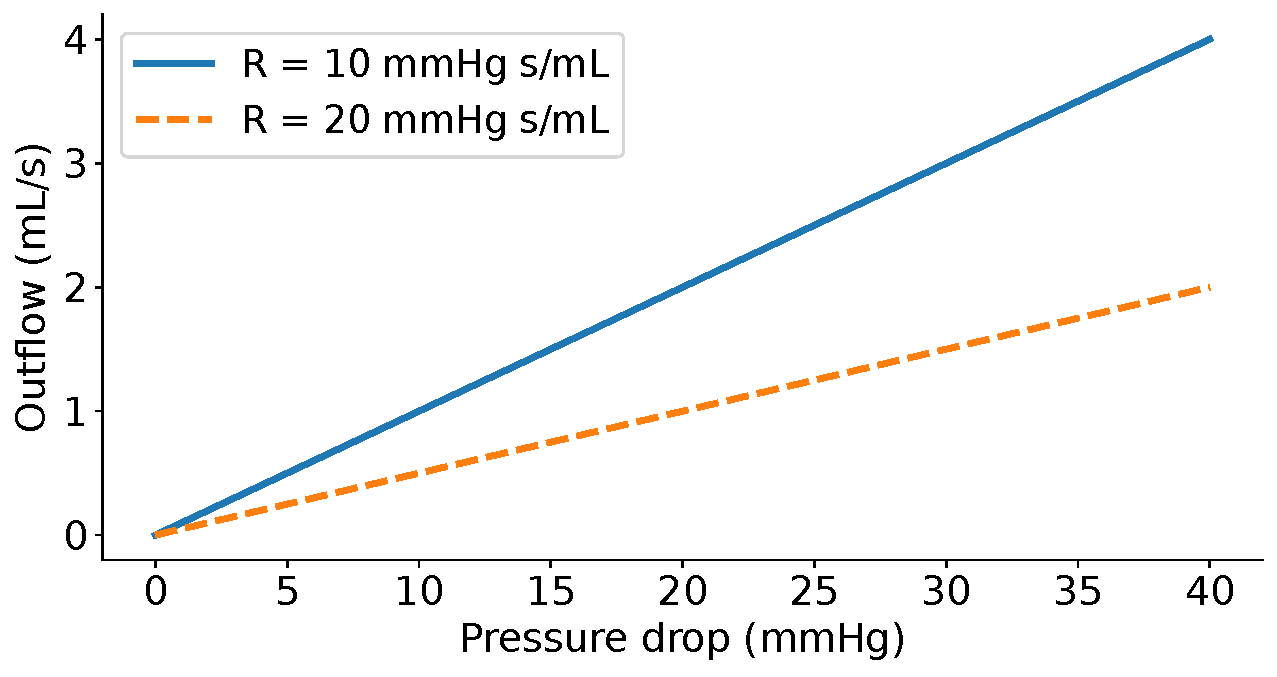
\includegraphics[width=.98\linewidth,height=.69\textheight,keepaspectratio]{presentation-figures/resistance-flow.pdf}\end{frame}
\renewcommand{\notestarget}{notes.pdf\#note-the-exponential-response}
\begin{frame}[label=slide-changing-compliance-panel-2]{Compliance and filling}
\centering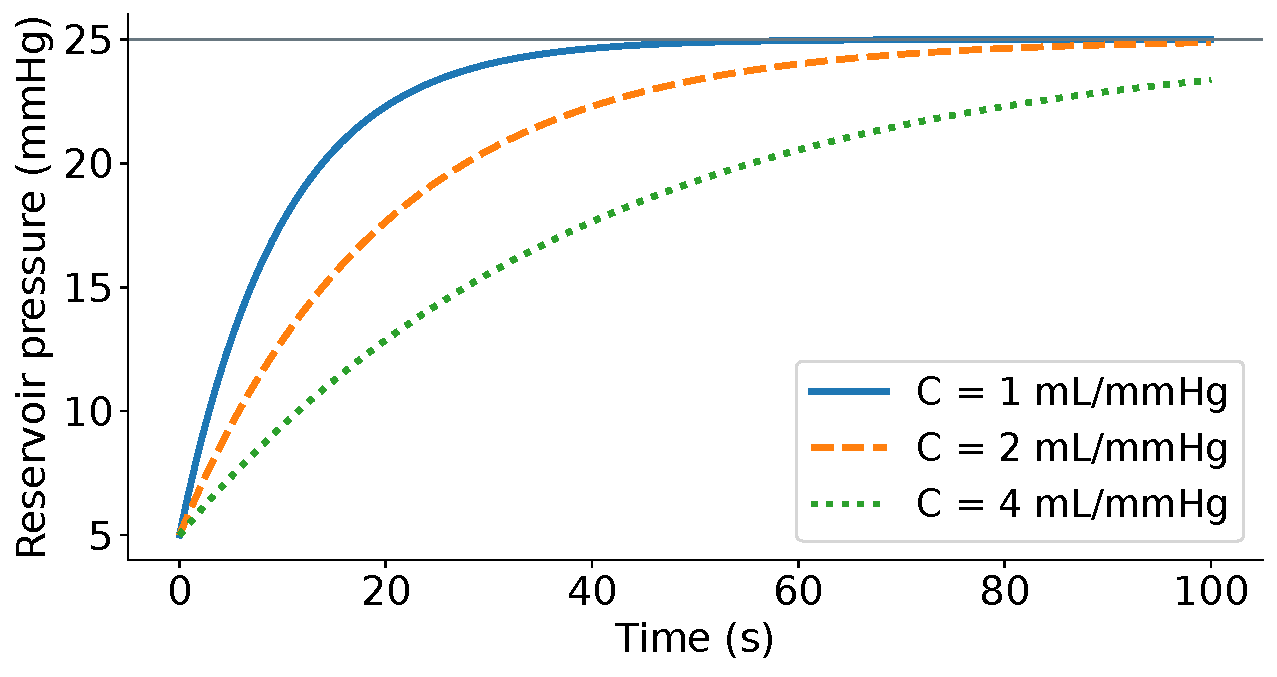
\includegraphics[width=.98\linewidth,height=.69\textheight,keepaspectratio]{presentation-figures/compliance-filling.pdf}\end{frame}
\renewcommand{\notestarget}{notes.pdf\#note-the-exponential-response}
\begin{frame}[t,fragile,label=slide-changing-compliance]{Changing compliance}
\[P_\infty=P_o+RI,\qquad \tau=RC.\]\pause{} At fixed $I,R,P_o$, increasing $C$ changes $\tau$ but leaves $P_\infty$ unchanged.
\end{frame}
\renewcommand{\notestarget}{notes.pdf\#note-spatial-resolution-and-the-question-being-asked}
\begin{frame}[t,fragile,label=slide-two-measurements-for-two-parameters]{Two measurements for two parameters}
\[R=\frac{P_\infty-P_o}{I}\quad(I\ne0),\qquad C=\frac\tau R.\]\pause{} A final pressure alone leaves compliance undetermined.
\end{frame}
\renewcommand{\notestarget}{notes.pdf\#note-spatial-resolution-and-the-question-being-asked}
\begin{frame}[label=slide-spatial-resolution-of-a-compartment-model-panel-1]{Compartment storage and mean pressure}
\centering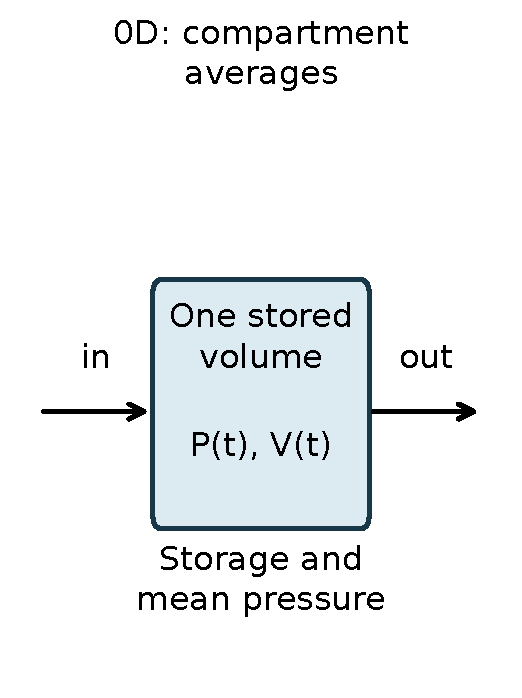
\includegraphics[width=.98\linewidth,height=.69\textheight,keepaspectratio]{presentation-figures/model-scale-0.pdf}\end{frame}
\renewcommand{\notestarget}{notes.pdf\#note-spatial-resolution-and-the-question-being-asked}
\begin{frame}[label=slide-spatial-resolution-of-a-compartment-model-panel-2]{Axial variation along a vessel}
\centering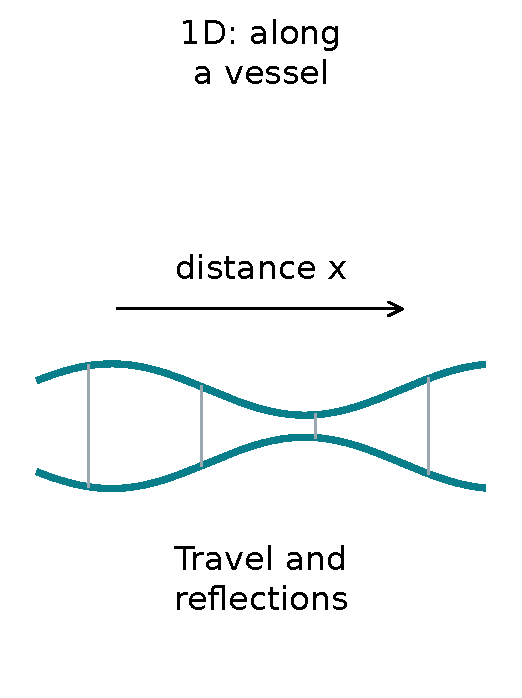
\includegraphics[width=.98\linewidth,height=.69\textheight,keepaspectratio]{presentation-figures/model-scale-1.pdf}\end{frame}
\renewcommand{\notestarget}{notes.pdf\#note-spatial-resolution-and-the-question-being-asked}
\begin{frame}[label=slide-spatial-resolution-of-a-compartment-model-panel-3]{Local flow and three-dimensional geometry}
\centering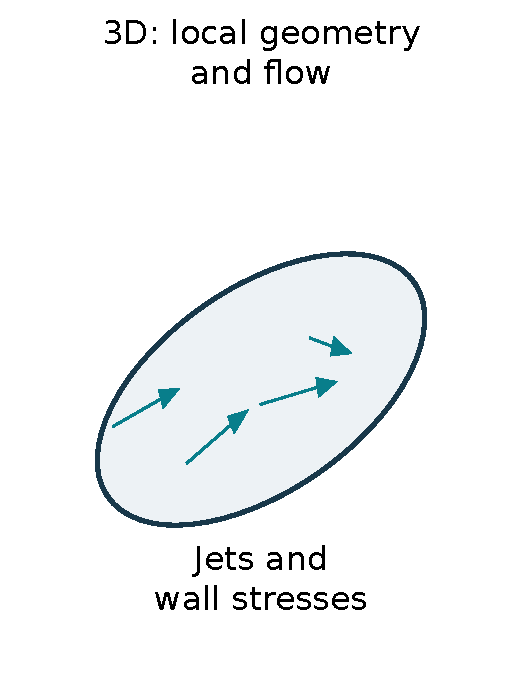
\includegraphics[width=.98\linewidth,height=.69\textheight,keepaspectratio]{presentation-figures/model-scale-2.pdf}\end{frame}
\renewcommand{\notestarget}{notes.pdf\#note-spatial-resolution-and-the-question-being-asked}
\begin{frame}[t,fragile,label=slide-spatial-resolution-of-a-compartment-model]{Spatial resolution of a compartment model}
0D: one compartment pressure and volume.\pause{}\par 1D: area and flow along a vessel.\pause{}\par 3D: a velocity field throughout local geometry.
\end{frame}
\renewcommand{\notestarget}{notes.pdf\#note-spatial-resolution-and-the-question-being-asked}
\begin{frame}[t,fragile,label=slide-a-model-can-pass-one-check-and-fail-another]{A model can pass one check and fail another}
The recurrence can conserve its volume balance while a large step gives an inaccurate trajectory.\pause{}\par The continuous formula can be computed exactly while the constant-compliance assumption fails experimentally.
\end{frame}
\end{document}
